\documentclass[9pt]{beamer}

\usepackage{booktabs}
\usepackage{geometry}
\usepackage{enumitem}

\usetheme{Copenhagen}

\title{Knowledge Grounding in Retrieval-Augmented LMs \\ Let's write a paper!}
\author{Martin Fixman et.\ al}
\institute{City, University of London}
\date{8 November 2024}

\begin{document}

\begin{frame}
	\titlepage{}
\end{frame}

\section{Timeline \& Journals}
\begin{frame}{Timeline \& Journals}
	Current goal: put the paper in a workshop \emph{as soon as possible}.

	\begin{itemize}
		\item ICLR workshop submission deadline: \textbf{April 27 2025}.
		\item ACL workshop submission deadline: \textbf{rolling deadline}.
	\end{itemize}
\end{frame}

\begin{frame}{Timeline \& Journals}
	Rough timeline:

	\begin{description}
		\item[6 December 2024] Next meeting.
			\begin{itemize}
				\item Most of the paper should be ready by now.
				\item I am going to Argentina shortly afterwards, but I will keep working there!
			\end{itemize}
		\item[April 27 2025] ICLR Workshop.
		\item[Later] Proper submission.
	\end{description}
\end{frame}

\section{Reading List}
\begin{frame}{Reading List}
	\begin{large}
		``Understanding the Interplay between Parametric and Contextual Knowledge for Large Language Models''
	\end{large} \\
	Cheng et.\ al

	\vfill{}

	\begin{center}
		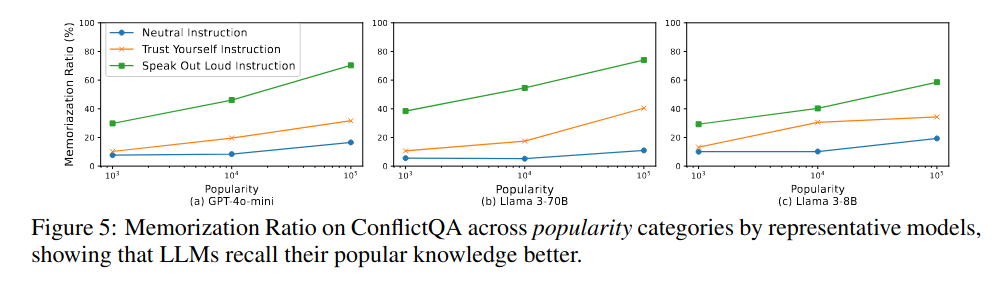
\includegraphics[width=\textwidth]{memorisation_ratio.png}
	\end{center}
\end{frame}

\section{Areas to expand in the paper}
\begin{frame}{Areas to expand in the paper}
	\begin{itemize}
		\item \textbf{Last minute additions}
			\begin{itemize}
				\item Attention part.
				\item Contextual-or-parametric classifier.
			\end{itemize}
		\item \textbf{Future work}
			\begin{itemize}
				\item Using ATLAS and similar models.
				\item Better categorisation of the answers.
				\item Natural Questions dataset.
			\end{itemize}
	\end{itemize}
\end{frame}

\end{document}
